%% This file is to be used as a template for your submission. 
%% Rename this file and replace the text with the text of 
%% your manuscript.
%%
%% The standard LaTeX document class "article" is recommended. 
%% Use options letterpaper and 12pt.
\documentclass[letterpaper,12pt]{article}

%% This is the recommended preamble for your document.

%% Load De Gruyter specific settings 
%\usepackage{dgjournal}

%% The mathptmx package is recommended for Times compatible math symbols.
%% Use mtpro2 or mathtime instead of mathptmx if you have the commercially
%% available MathTime fonts.
%% Other options are txfonts (free) or belleek (free) or TM-Math (commercial)
\usepackage{mathptmx}

%% Use the graphics package to include figures
\usepackage{graphics}

%% Use natbib with these recommended options
\usepackage[authoryear,comma,longnamesfirst,sectionbib]{natbib} 

%\usepackage{cite} % Make references as [1-4], not [1,2,3,4]
\usepackage{url}  % Formatting web addresses  
\usepackage{ifthen}  % Conditional 
\usepackage{multicol}   %Columns
\usepackage[utf8]{inputenc} %unicode support
\usepackage{amsmath}
\usepackage[pdftex]{graphicx}
%\usepackage{hyperref}
\usepackage{subfigure}
\usepackage{xcolor}
\usepackage[normalem]{ulem} % 
\usepackage{authblk}

\title{Model selection for prognostic time-to-event gene signature discovery with applications in early breast cancer data}
%\abstract{}
\author[1]{Miika Ahdesm\"aki}
\author[1]{Lee Lancashire}
\author[1]{Vitali Proutski}
\author[1]{Claire Wilson}
\author[1]{Timothy Davison}
\author[1,2]{D. Paul Harkin}
\author[1,2]{Richard Kennedy}
\affil[1]{Almac Diagnostics, 19 Seagoe Industrial Estate, BT63 5QD Craigavon, United Kingdom}
\affil[2]{Queen's University of Belfast, Centre for Cancer Research and Cell Biology, BT9 7BL Belfast, United Kingdom}

%% Start your document body here
\begin{document}
\maketitle

\begin{abstract}
Model selection between competing models is a key consideration in the
discovery of prognostic multigene signatures. The use of appropriate
statistical performance measures as well verification of biological
significance of the signatures is imperative to maximise the chance of
external validation of the generated signatures. Current approaches in
time-to-event studies often use only a single measure of performance in
model selection, such as logrank test p-values, ordichotomise the follow-
up times at some phase of the study to facilitate signature discovery. In
this study we improve the prognostic signature discovery process through
the application of the multivariate partial Cox model combined with the
concordance index, hazard ratio of predictions, independence from
available clinical covariates and biological enrichment as measures of
signature performance. The proposed framework was applied to discover
prognostic multigene signatures from early breast cancer data. The partial
Cox model combined with the multiple performance measures were used in
both guiding the selection of the optimal panel of prognostic genes and
prediction of risk within cross validation without dichotomising the follow-
up times at any stage. The signatures were successfully externally cross
validated in independent breast cancer datasets, yielding a hazard ratio of
2.55 [1.44, 4.51] for the top ranking signature. 
\end{abstract}

\section{Introduction}
In cancer medicine it is increasingly appreciated that tumours arising from the same anatomical site in different patients can represent distinct diseases at a molecular level. Advances in mRNA, miRNA and DNA analysis have allowed the classification of tumours at a molecular level and have the promise of guiding personalised treatment strategies. The largest impact is likely to be in the discovery of prognostic assays, which predict outcome in the absence of a specific treatment, and predictive assays that predict the outcome following a specified therapy. Gene expression microarrays have been at the forefront of complex analysis of tumour biology as they are able to capture the relative expression of tens of thousands of genes simultaneously. In addition, they represent a mature diagnostic platform with demonstrated clinical applicability and suitable performance for in-vitro-diagnostic regulatory approval (\citet{Veer:02,Pillai:11}).

In prognostic studies, where follow-up times are monitored instead of a binary outcome, the time to event data is typically analysed using Cox proportional hazards regression. An issue with this approach when applied to high throughput genomic data is multidimensionality where the number of genes analysed greatly exceeds the number of samples. Although modifications for analysing high dimensional data have been proposed for the Cox model (\citet{Boulesteix:06, Li:04, Gui:05, Witten:10}) and survival analysis for random forests (\citet{Ishwaran:08}), time-to-event models for prediction have not been widely adopted in prognostic biomarker signature research. In fact, many prognostic signature discovery studies do not utilise time-to-event analysis algorithms at all (see e.g.\ \citet{Schmidt:08}) or use Cox regression for ranking the genes but dichotomise the follow-up times to estimate binary performance measures such as area under the ROC curve (see e.g.\ \citet{Wang:05}). In one exception, Kammers and co-authors used Lasso penalised Cox regression to analyse two microarray data sets and reported the prognostic index and Brier scores for the predictions (\citet{Kammers:11}). 

The main contribution of this article is to introduce a completely continuous framework with performance measures for model selection that do not dichotomise the follow-up times at any stage. To this end, we use partial Cox regression combined with the concordance index (Harrell's c-index (\citet{Harrell:10,Raykar:07})) and hazard ratio based performance evaluation of the risk scores and follow-up times for the discovery of the optimal panel of prognostic genes. The c-index has been recommended as a general measure of the predictive power of prognostic biomarkers (\citet{Newson:06}). It estimates the probability of concordance between predicted and observed time to event, with $0.5$ for random predictions and $1$ for predictions matching the order of observed event times (\citet{Harrell:10}). For binary responses it is equivalent (\citet{Newson:06}) to the area under the receiving operator characteristic curve (AUC), a frequently used measure in binary classification problems. In addition, when selecting for the optimal signature among the generated signatures, we analyse the results for biological relevance and independence from technical and clinical covariates thereby ensuring clinical applicability. We present semi-automatic signature generation methods that follow the general guidelines of the Microarray Quality Control (MAQC) Consortium and have been designed with clinical utility in mind. We use this methodology to discover multigene signatures that predict risk of distant metastasis in early breast cancer and successfully validate in independent datasets.



\section{Methods}
\subsection{Data sets}
Three datasets with an endpoint defined by breast cancer distant metastasis were downloaded. These datasets included the GSE11121\footnote{http://www.ncbi.nlm.nih.gov/geo/query/acc.cgi?acc=gse11121} Mainz study (\citet{Schmidt:08}, also analysed in \citet{Kammers:11}), the GSE2034\footnote{http://www.ncbi.nlm.nih.gov/geo/query/acc.cgi?acc=gse2034} Rotterdam study (\citet{Wang:05}) and the GSE7390\footnote{http://www.ncbi.nlm.nih.gov/geo/query/acc.cgi?acc=gse7390} TRANSBIG breast cancer study (\citet{Desmedt:07}). In the TRANSBIG data, all events after $10$ years were censored, as in the original publication. The effect of this additional censoring is studied in more detail in the results section. Each of these three data sets were used once as training sets and the two remaining ones as external validation sets, composing a 3-by-3 table of results (Table \ref{Table:HRTable2}). The samples were all profiled on the Affymetrix HG-U133A platform, containing $247965$ probes that can be summarised further to $22283$ probesets. These probesets roughly map to one or more human transcripts and represent a snapshot of expressed transcripts in the samples.

A summary of the data sets is given in Table \ref{Table:DataSets}. Note that the number of events for the TRANSBIG data was 62 in the original database but after censoring samples with more than $10$ years of follow-up (as suggested in \citet{Desmedt:07}) this was reduced to $50$. In the available clinical covariates considered for confounding effects, missing values were replaced by median of the present values. Multilevel nominal covariates were represented by $N-1$ binary indicators, where $N$ is the number of levels in a given covariate. Covariates with underrepresented levels were discarded. In the clinical data for the TRANSBIG study, lymphocytic infiltration and angioinvasion contained too many missing values and were excluded. All of the breast cancer samples in these datasets were lymph node negative.


% TRANSIBG: Hospital, Age, Size, Surgery, Histology, Grade, ER+
% MAQC: Age, Sex, Race, Isotype, B2M, CRP, Creat, LDH, ALB, HGB, ASPC, BMPC, MRI
\begin{table}[h]
\centering
\caption{Summary of the data sets used in this paper. ER+ stands for estrogen receptor positive indicator. The data set identifiers are further explained under subsection Data sets.}
\label{Table:DataSets}
\begin{small}
    \begin{tabular}{ | l | c | c | c | l |} 
    \hline
    Data set & Samples & Events & Median & Clinical \\ &&& follow-up & covariates \\&&& time & \\ \hline \hline
    GSE2034 HG-U133A		& 286 	& 107 & 86 mo & ER+\\ 
		Rotterdam &&&& Brain relapse\\\hline
		GSE7390 HG-U133A		& 198 	& 50 	& 144.1 mo & Hospital \\ TRANSBIG  &&&& Age\\ &&&& Size\\&&&& Surgery\\&&&& Histology\\&&&& Grade\\&&&& ER+\\\hline
		GSE11121 HG-U133A		& 200 	& 46 	& 90.5 mo & Grade\\ 
		Mainz cohort &&&& Size\\\hline
    \end{tabular}
\end{small}
\end{table}


\subsection{Pre-processing and exploratory analysis}
To enable a multisample, multivariable analysis of the microarray data sets, pre-processing of the data including background correction, normalisation and probeset summarisation was first considered to ensure comparability of the gene expression levels. One option would be to combine all the chosen data sets and pre-process them together. However, due to the chosen pre-processing being multichip (see below), this approach would not be feasible if the signature was taken to clinic due to new samples coming in one at a time. Using validation samples together with the model training samples in multichip pre-processing would also introduce a positive bias similar to using validation samples as part of a training set when building a predictive model.
All samples were independently background corrected per array using the per-sample background correction algorithm in Robust Multichip Average (RMA, \citet{Bolstad:03}), the widely accepted pre-processing tool for gene expression microarray data. Each of the training sets were quantile normalised and median polish summarised using RMA. The quantiles from training set normalisation and probe affinities from summarisation were then applied to the corresponding external validation or cross-validation test sets one sample at a time (Reference RMA, \citet{Katz:06}). Affymetrix control probesets were discarded after probeset summarisation. 

The concept of classification difficulty estimation was introduced in \citet{Popovici:10} for the purpose of exploring associations between variables and a binary endpoint. In brief, for each probeset a squared t-score is evaluated and the cumulative sum of the ordered squares is plotted to evaluate whether or not there is a strong association between the endpoint values and the data. For time-to-event analysis, we instead plot the cumulative sum of the ordered absolute univariate Cox coefficients. The cumulative sum is additionally compared to a negative control distribution obtained by permuting the follow-up time values of the samples along with their event indicators. In general, in both classification and Cox model difficulty estimation the resulting curve is monotonously increasing approaching a plateau after the most informative variables have been added (see Figure \ref{Fig:DifficultyPlots} for an example). For the Cox model difficulty estimation the RMA pre-processed probesets were filtered by 50\% based on low variance and intensity (see \cite{Hackstadt:09} for motivation) as within the actual signature discovery, see details below.


\subsection{Prognostic signature generation}
In evaluating the generalisation performance and optimal length of the signatures, each of the training data sets was split into $5$ folds of cross-validation repeated $10$ times, with stratification such that the proportion of events and distributions of follow-up times were approximately equal between each fold of the cross-validation training sets and the full training set. Each cross-validation training set was normalised (quantile normalisation, storing the training set quantiles) and summarised (median polish, storing the estimated probe affinities) and the obtained pre-processing models were applied to the cross-validation test sets. Analogously, the ref-RMA pre-processing models from the full training sets were eventually used to pre-process the validation sets sample by sample. It is emphasised that cross-validation was used to guide in the selection of the optimal signature length only and not for the training of any final signature per se. The final signatures were trained by repeating the feature selection process in the full training sets (see \citet{Simon:12} for motivation).

Within each cross-validation training set, the probesets were filtered by 50\% based on variance and intensity (\citet{Hackstadt:09}). Average rank of high variance and high intensity was used in the filter, retaining the highest ranked variables. To further lessen the computational burden within feature selection and to reduce the number of null variables, the probesets were further filtered down to approximately $1000$ probesets using a univariate Cox filter, based on the Cox proportional hazards (PH) model coefficients from univariate analyses of the probesets. This second filtering step is by no means obligatory and the presented feature selection method is not limited to starting with 1000 features should sufficient computational resources be available. Both of these hard thresholds (50\% followed by down to approximately $1000$ covariates) were chosen instead of for example controlling for false discovery rate (FDR) in the filtering to ensure a consistent starting size of probesets for the feature selection for all folds and repeats of cross-validation. For the remaining probesets, an iterative backwards elimination feature selection procedure was applied using 3-component partial Cox regression (\citet{Li:04}), where the partial Cox coefficients of the probesets were used for ranking (see Figure \ref{Fig:SignGenFlowchart}). During each iteration, 10\% of the lowest ranking probesets were discarded after predicting the cross-validation test set risk scores (see Eq.\ \ref{eq:riskScore} for the definition of the risk score). No information leakage was allowed from the cross-validation test set, i.e.\ the probeset ranking was purely based on the coefficients from the cross-validation training set. This procedure was repeated until five probesets remained. The c-index (\citet{Harrell:10}, see Eq.\ \ref{eq:Cindex}) of the continuous cross-validation test set risk score predictions was evaluated as the main performance measure. Additionally, univariate hazard ratios of the cross-validation test set risk scores, dichotomised at risk score value $0$ (Eq.\ \ref{eq:dichRiskScore}, i.e. low risk $<0$, high risk $>0$, \citet{Li:04}), were evaluated. The process is summarised in Figure \ref{Fig:SignGenFlowchart}.

\begin{figure}[!th]
\centering
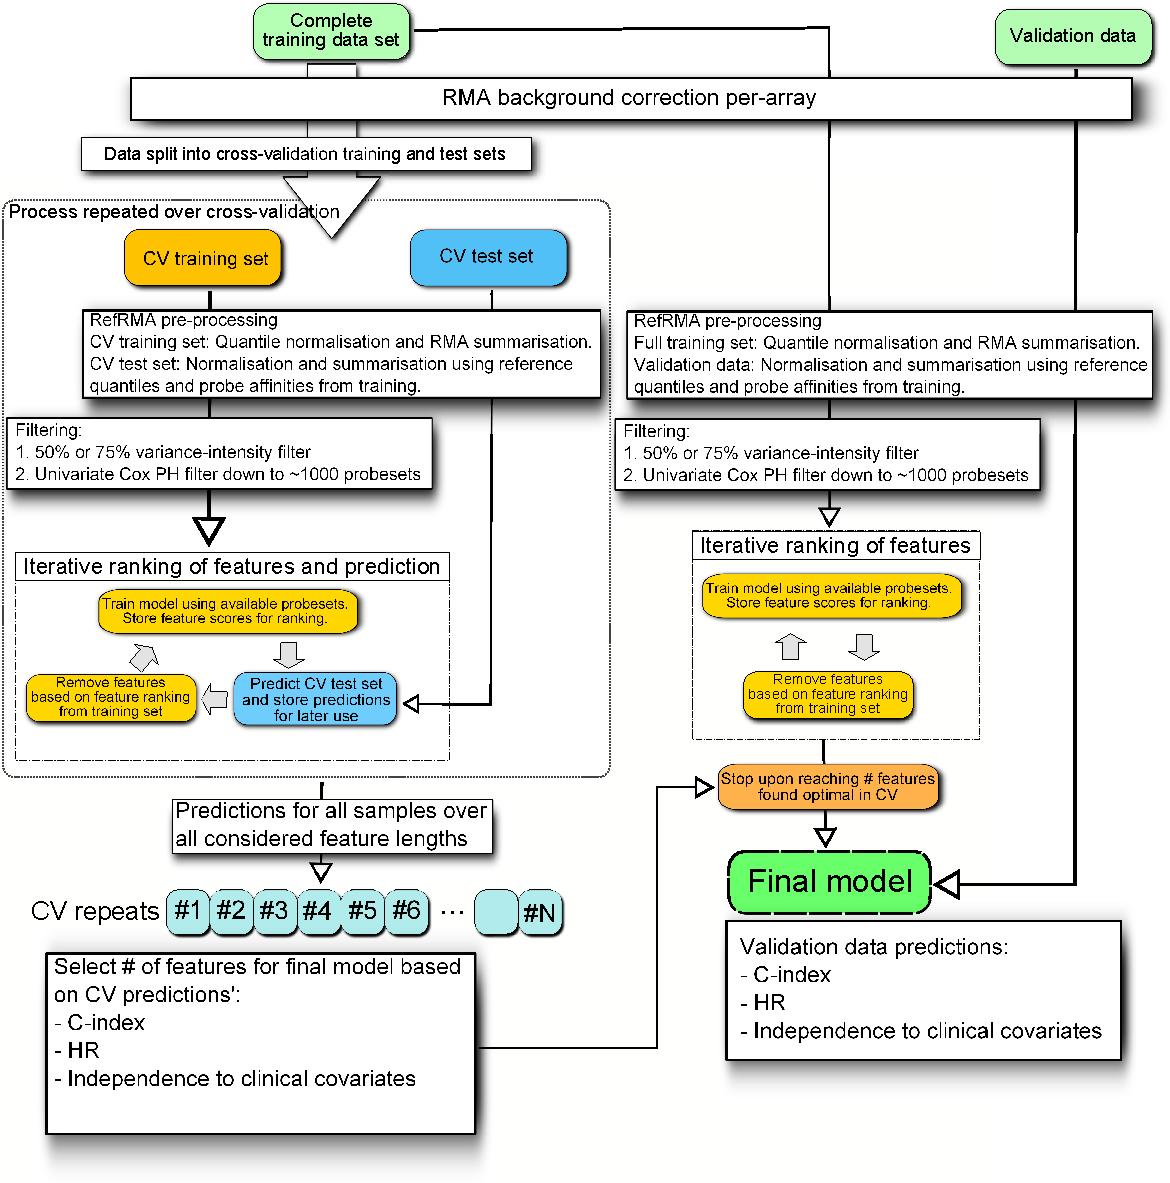
\includegraphics[scale=0.30]{Figures/WorkflowOverview.jpeg}
\caption{Flowchart of the signature generation and evaluation process.}
\label{Fig:SignGenFlowchart}
\end{figure}

When deciding on the signature length, the signature lengths that maximise the HR and c-index in cross-validation may not necessarily be the same. To aid in model selection, independence to clinical covariates was also evaluated within cross-validation. A generalised Cox PH likelihood ratio test (Eq.\ \ref{eq:LRtest}) was used to this end in which a full model with dichotomised predictions and clinical covariates is compared to a reduced model with the clinical covariates only in predicting time to event. 

In addition, signatures with the minimal number of probesets possible whilst maintaining performance were favoured. We suggest that the feature length selection step requires human guidance as different objectives could influence the selection of the feature length, such as desire to migrate to another platform, error interval width and so on.  Additionally, in the case where the selection is somewhat arbitrary, due to the similarity of the different performance measures, any feature length with comparable performance could be selected, and the one chosen and reported on here is only as an example. As a compromise, maximum signature length was set to $600$ (\citet{Kennedy:11} used $634$ probesets) and the signature length below $600$ that maximised the c-index was chosen unless other criteria showed poor results for the same length.

To summarise generic model selection criteria for time-to-event and to aid the more inexperienced researchers in comparing competing models, we list here our recommendations for selecting between models, in order of importance:
\begin{enumerate}
  \item Select the signature that maximises the (average) concordance index within cross-validation and whose error bars or confidence interval does not overlap the 50\% limit.
  \item Select the signature that maximises the hazard ratio and whose error bars or confidence interval does not overlap one. 
  \item If clinical and / or technical confounder information is available, select the signature whose p-value in a Cox model likelihood ratio test of independence to the confounders is the lowest.
  \item If none of the above criteria can distinguish between the highest ranking signatures, observe if biological processes related to the disease under study are more enriched in one signature versus another.
\end{enumerate}
Our recommendations are based on our extensive experience in working with predictive classifier models where the analysis of the models is driven by AUC, whose extension into the time-to-event case the c-index is. However it is often required to select a signature score dichotomisation threshold for binary classifier models afterwards to enable estimation of sensitivity, specificity, NPV and / or PPV. In these cases the serial process is AUC based model selection followed by threshold selection driven by clinical utility (e.g.\ a fixed specificity). In the time-to-event space this is akin to using the c-index as a primary measure for model selection followed by HR estimation. In both domains a likelihood ratio test can be used to assess independence from clinical and / or technical covariates (logistic regression in binary classification and Cox model in time-to-event). 

The partial Cox regression algorithm (\citet{Li:04}) was chosen for the biomarker discovery analyses because it is theoretically based on the same idea as partial least squares (PLS) regression, an established method in high dimensional analyses (\citet{Boulesteix:06}). It is also analogous to principal components analysis in that the first few latent components explain most of the information in the data. Additionally, partial Cox requires no parameter tuning in nested cross-validation and therefore the computational complexity is modest compared to the Lasso Cox approach taken by the authors in \citet{Kammers:11}. 

Due to the public unavailability of the original implementation, Partial Cox regression will be made available in R from the package \verb1PartialCox1. The c-index and many other useful functions are available in the package \verb1Hmisc1 .


\subsection{Definitions of important parameters and statistics}
The risk score used in this publication is defined as the linear combination of the signature probeset values multiplied by their corresponding partial Cox model coefficients, first subtracted by the training set probeset mean values (see \citet{Li:04} for the Cox model and risk score definitions):
\begin{equation}
y^{new} = (\mathbf{x}^{new}-\overline{\mathbf{x}}^{train})^{\prime} \hat{\mathbf{\beta}},
\label{eq:riskScore}
\end{equation}
where $y^{new}$ is the continuous risk score for the new sample, $\mathbf{x}^{new}$ is the vector of individual probeset values for the new sample, $\overline{\mathbf{x}}^{train}$ is the vector of probeset mean values from the training set and $\hat{\mathbf{\beta}}$ are the partial Cox model coefficients from training.

The risk scores have by definition a sample mean of zero \citet{Li:04}, and dichotomisation of the risk scores for hazard ratio calculation is obtained via the indicator function,
\begin{equation}
I_{y^{new}>0},
\label{eq:dichRiskScore}
\end{equation}
which equatos to one for positive values and zero otherwise.

The hazard ratio of predictions is given by
\begin{equation}
e^{b_p},
\end{equation}
where $b_p$ is the Cox model coefficient from a Cox model when modelling survival time by the dichotomised signature risk scores. 

The concordance index is best understood by considering the ordered follow-up times as a directed graph, as in \citet{Raykar:07}. The total number of edges in the ordered follow-up time graph depends mainly on the number of events, as an edge is drawn only from events to any event or censoring having a follow-up time greater than that of the event considered. The concordance index is obtained by counting the number of edges in the graph where the predicted survival times for the samples agree with the direction of the edges, divided by the total number of edges:
\begin{equation}
c=\frac{1}{|\varepsilon |}\sum_{T_i~\text{uncensored} }\sum_{T_j > T_i}1_{f(x_i)<f(x_j)},
\label{eq:Cindex}
\end{equation}
where $\varepsilon$ denotes the total number of edges in the graph, $T_i$ are the follow-up times, $f(x_i)$ are the predicted survival times and $1_{f(x_i)<f(x_j)}$ is an indicator variable that is one when ${f(x_i)<f(x_j)}$ is true, zero otherwise. The risk scores have an inverse relationship with predicted survival times, i.e.\ high risk score implies low predicted survival time. Therefore, for risk scores, $f(x_i)<f(x_j)$ in Eq.\ \ref{eq:Cindex} needs to be replaced by $f_{risk}(x_i)>f_{risk}(x_j)$.

The likelihood ratio statistic used in evaluating the effect of clinical covariates (confounders) is given by
\begin{equation}
-2\left(\ln\hat{L}_{reduced} - \ln\hat{L}_{full} \right) \sim \chi^2_1
\label{eq:LRtest}
\end{equation}
where the Cox model log-likelihoods ($\ln\hat{L}$) and chi-square distribution values can readily be obtained from standard statistical software packages. The degrees of freedom default to one as the model order difference is always one here.



\section{Results}
\subsection{Prognostic signature generation results}
Three datasets were selected to test our methodology. The Mainz dataset (\citet{Schmidt:08}) consists of microarray data from $200$ lymph node negative, ER positive (ER+ve) and negative (ER-ve) patients who did not receive systemic adjuvant therapy. The number of metastatic recurrences recorded was $46$, $18$ of which were beyond five years. The Rotterdam dataset (\citet{Wang:05}) consists of microarray data from $286$ lymph node–negative ER+ve and ER-ve patients who did not receive adjuvant systemic therapy. Ninety three metastatic recurrences were reported, although no data is available after five years. Finally the TRANSBIG study (\citet{Desmedt:07}) consists of microarray data from $198$ ER+ve and ER-ve patients who also did not receive adjuvant systemic therapy after surgery. Fifty patients developed metastatic recurrence before ten years of which $14$ occurred after five years. Importantly, these datasets are entirely independent and therefore ideal for testing our methodology for identifying and validating clinically meaningful prognostic signatures. Although microarray data is used here solely, the proposed methodology is applicable to other high dimensional data equally well.

Analysis of associations between predictors (probesets in case of Affymetrix microarrays) and time to distant metastasis for each of the three training sets revealed that the association between the data and survival time (time to distant metastasis) is stronger than expected by chance. This is shown by the thick solid curve being above the 97.5\% quantile (upper dashed line) of the negative control distribution (Figure \ref{Fig:DifficultyPlots}).

%%%%%%%%%%%%%%%%%%%
%%%%%%%%%%%%%%%%%%%
%%%%%%%%%%%%%%%%%%%
% difficulty plots
\begin{figure}[!th]

\centering
\subfigure[Mainz]{
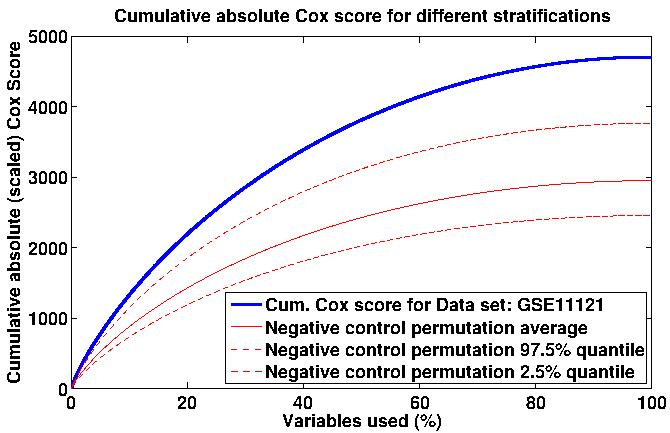
\includegraphics[width=0.48\textwidth]{Figures/Mainz_CoxDifficulty.jpeg}
\label{fig:subfig2}
}
\subfigure[Rotterdam]{
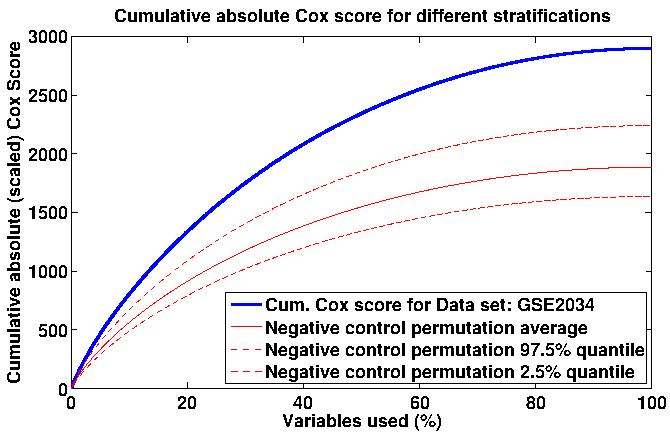
\includegraphics[width=0.48\textwidth]{Figures/Wang_CoxDifficulty.jpeg}
\label{fig:subfig3}
}
\subfigure[TRANSBIG]{
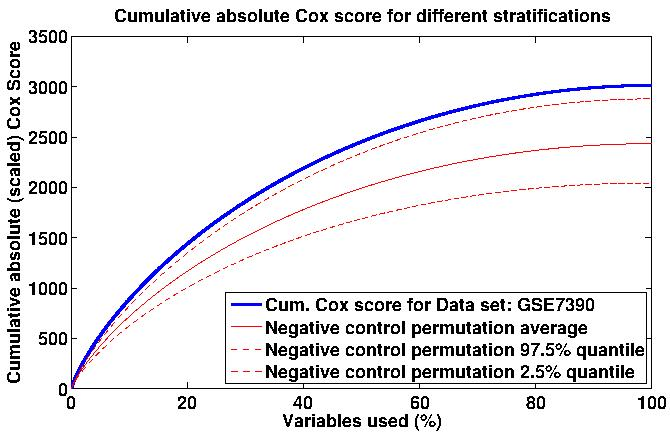
\includegraphics[width=0.48\textwidth]{Figures/Transbig_CoxDifficulty.jpeg}
\label{fig:subfig4}
}
\caption{Cox model generation difficulty estimate plots. X-axis shows the percentage probesets included in the cumulative sum. Permutation based negative control distribution quantiles are plotted in dashed lines.}
\label{Fig:DifficultyPlots}
\end{figure}


Signature generation and evaluation was then performed (summarised in Figure \ref{Fig:SignGenFlowchart}). The test set prediction results from all the ten cross-validation repeats are shown in Figures \ref{Fig:PLSCoxCindex} (c-index), \ref{Fig:PLSCoxHR} (HR) and \ref{Fig:PLSCoxIndep} (minus $\log_{10}$ p-values of independence to clinical covariates) for the different training data sets. A decreasing trend in performance can be observed towards the shorter signature lengths, with the minus log p-values (Figure \ref{Fig:PLSCoxIndep}) following the same trends as the HR (Figure \ref{Fig:PLSCoxHR}). There was clearly no steep drop in performance at any signature length, therefore leading to an amount of redundancy in selecting the optimal feature length. As different studies have different objectives, e.g.\ it might be required to optimise the signature for maximum hazard ratio, to minimise error bars or limit the number of genes to less than 20 to enable migration to qPCR, all this information must be considered in a human decision guided fashion. Here emphasis was placed such that signature lengths that maximise the c-index below $600$ variables are highlighted for the results from the Mainz and Rotterdam datasets, whereas for the TRANSBIG results the highlighted signature length ($252$) maximises HR and gives a good compromise on c-index.


%%%%%%%%%%%%%%%%%%%
%%%%%%%%%%%%%%%%%%%
%%%%%%%%%%%%%%%%%%%
%
% c-index
%

\begin{figure}[!th]
\centering

\subfigure[Mainz]{
%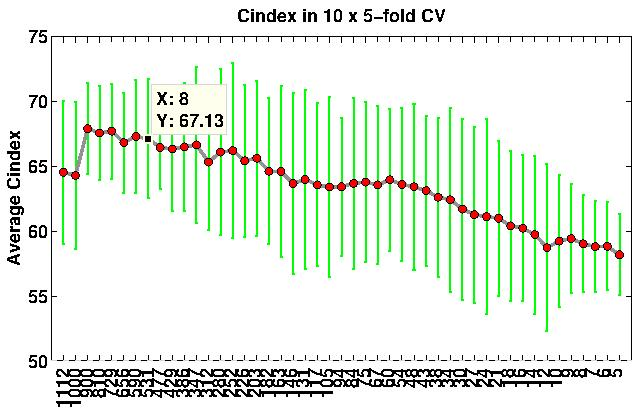
\includegraphics[scale=0.37]{Figures/Mainz_Cindex.jpeg}
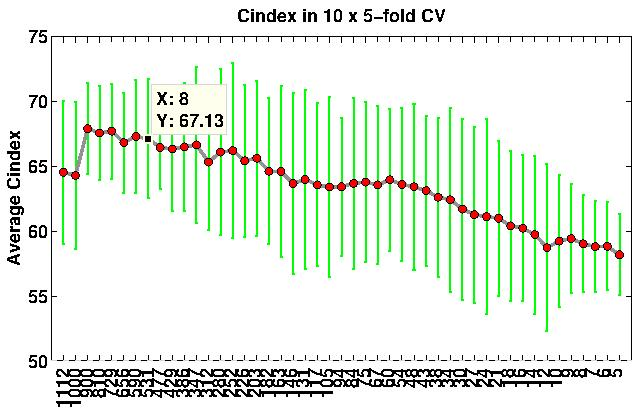
\includegraphics[width=0.6\textwidth]{Figures/Mainz_Cindex.jpeg}
\label{fig:Csubfig2}
}
\subfigure[Rotterdam]{
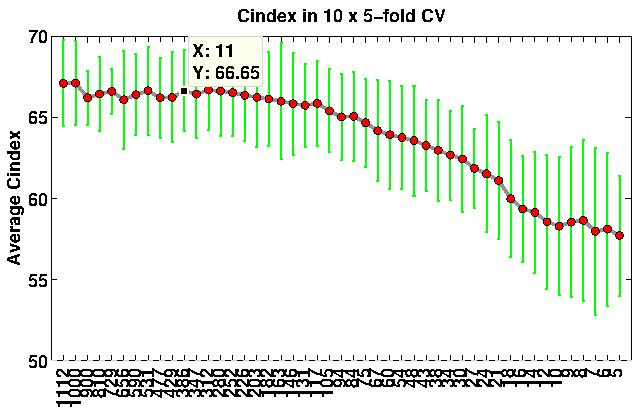
\includegraphics[width=0.6\textwidth]{Figures/Wang_Cindex.jpeg}
\label{fig:Csubfig3}
}
\subfigure[TRANSBIG]{
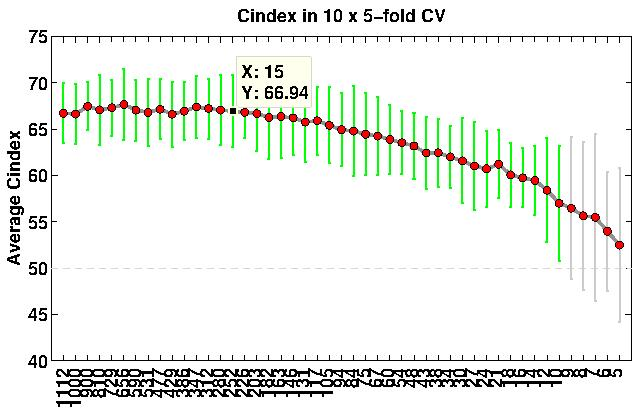
\includegraphics[width=0.6\textwidth]{Figures/Transbig_Cindex.jpeg}
\label{fig:Csubfig4}
}
\caption{Concordance index summaries over considered feature lengths and cross-validation repeats. Means (circles) of the ten cross-validation repeats are plotted with the two standard deviation (2SD) based prediction intervals. Dashed gray line corresponds to concordance index of 0.5. Y-axis: c-index for the cross-validation test set predictions. X-axis: Probeset lengths evaluated.}
\label{Fig:PLSCoxCindex}
\end{figure}

%
% HR
%
\begin{figure}[!th]

\centering
\subfigure[Mainz]{
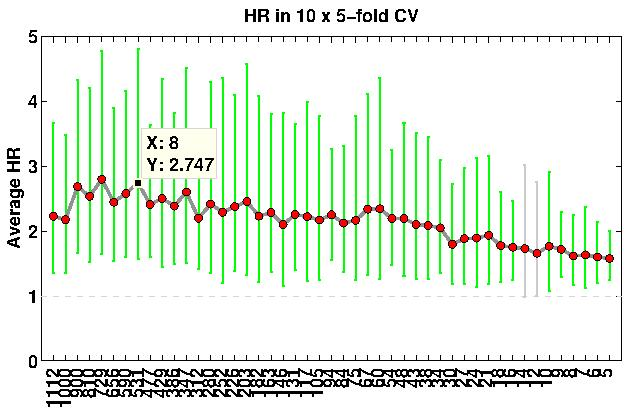
\includegraphics[width=0.6\textwidth]{Figures/Mainz_HR.jpeg}
\label{fig:HRsubfig2}
}
\subfigure[Rotterdam]{
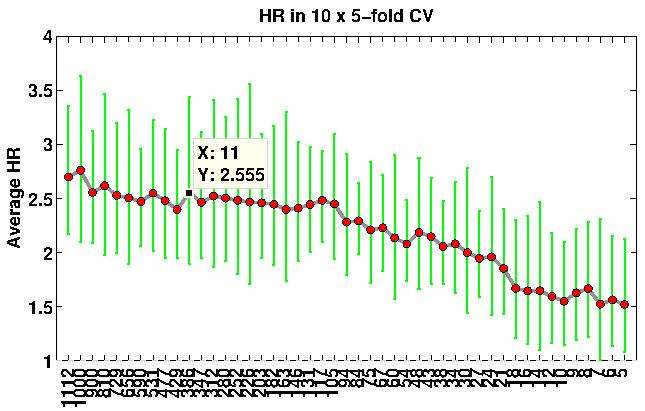
\includegraphics[width=0.6\textwidth]{Figures/Wang_HR.jpeg}
\label{fig:HRsubfig3}
}
\subfigure[TRANSBIG]{
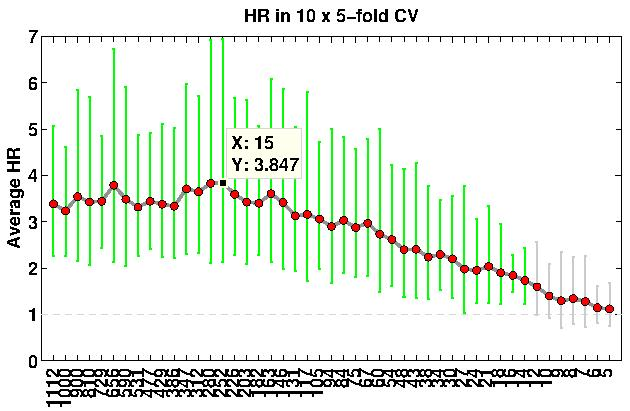
\includegraphics[width=0.6\textwidth]{Figures/Transbig_HR.jpeg}
\label{fig:HRsubfig4}
}
\caption{Hazard ratio summaries over considered feature lengths and cross-validation repeats. The means (circles) and 2SD intervals were evaluated on the natural logarithmic scale and then exponentiated back to original scale. Dashed gray line corresponds to HR of 1. Y-axis: Hazard ratios of dichotomised cross-validation test set predictions. X-axis: Probeset lengths evaluated.}
\label{Fig:PLSCoxHR}
\end{figure}
%
% independence to clinical covariates
%
\begin{figure}[!th]

\centering
\subfigure[Mainz]{
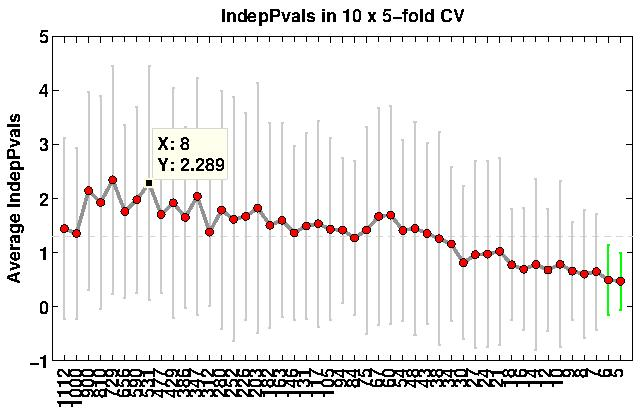
\includegraphics[width=0.6\textwidth]{Figures/Mainz_ClinIndepP.jpeg}
\label{fig:pvalsubfig2}
}
\subfigure[Rotterdam]{
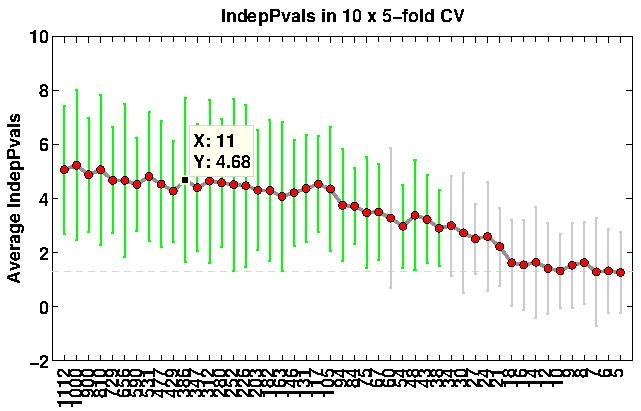
\includegraphics[width=0.6\textwidth]{Figures/Wang_ClinIndepP.jpeg}
\label{fig:pvalsubfig3}
}
\subfigure[TRANSBIG]{
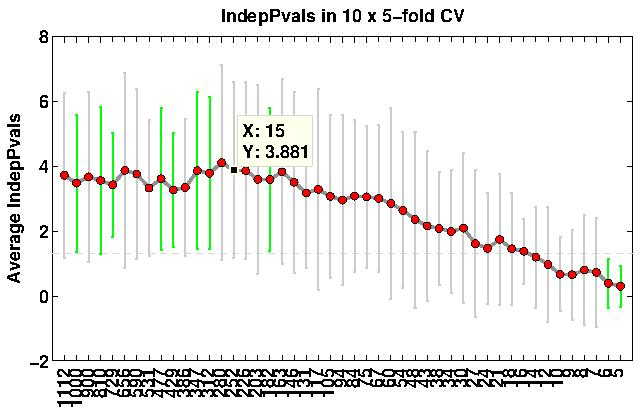
\includegraphics[width=0.6\textwidth]{Figures/Transbig_ClinIndepP.jpeg}
\label{fig:pvalsubfig4}
}
\caption{Minus log10 p-value summaries from likelihood ratio testing of importance of the predictions given the clinical covariates. Dashed gray line corresponds to 0.05 level on the log-scale. Y-axis: Mean minus log10 p-values of the cross-validation test set predictions. X-axis: Probeset lengths evaluated.}
\label{Fig:PLSCoxIndep}
\end{figure}


Final prognostic signatures for each data set were generated by repeating the iterative feature selection process on the respective full data set. Final partial Cox models were trained at the chosen feature lengths (Mainz: 531, Rotterdam: 386, TRANSBIG: 252). For average performance of signatures of these lengths in cross-validation see the diagonal entries of Table \ref{Table:HRTable2}. The overlap of the final signature probesets for the three breast cancer signatures is depicted in a Venn diagram (Figure \ref{Fig:Venn3}). The small observed overlap in the probesets comprising the three signatures shows that there is clearly some redundancy in which probesets to choose to predict the same endpoint, as the signatures largely validate across the data sets (see Prognostic signature validation results below). 

%%%%%%%%%%%%%%%%%%%%%%%%%%%
%%%%%%%%%%%%%%%%%%%%%%%%%%%

\begin{table}[h]
\centering
\caption{Performance measures for the breast cancer distant metastasis cross-validation test (diagonal) and validation set (off-diagonal) predictions. 'C' denotes concordance index, 'HR' hazard ratio, 'CI' the 95\% confidence interval (validation sets only), 'HR p-val' the p-value for testing HR=1 (validation sets only) and 'PH p-val' the p-value for testing the proportional hazards assumption with a low value implying a violation (validation sets only). The values on the diagonal represent average performance in cross-validation.}
\label{Table:HRTable2}
\begin{small}
    \begin{tabular}{ | l r | l | l | l |} 
    \hline
     & Model & Mainz & Rotterdam & TRANSBIG \\ Data & & 531PS & 386PS & 252PS \\\hline \hline
    Mainz & C [CI]:& 0.671& 0.629 [0.540, 0.708]& 0.613 [0.517, 0.703]\\ &HR [CI]:& 2.75 & 2.04 [1.13, 3.68]&1.66 [0.86, 3.20]\\ &HR p-val:& & 0.018&0.134\\ &PH p-val& & 0.027& 0.005\\\hline
		Rotterdam  & C [CI]:& 0.617 [0.562, 0.667]& 0.667& 0.610 [0.555, 0.659]\\ &HR [CI]:& 2.09 [1.37, 3.19]& 2.56 &1.71 [1.00, 2.91]\\ &HR p-val:& 0.0006&&0.049\\ &PH p-val& 0.084& & 0.112\\\hline
		TRANSBIG  & C [CI]:& 0.648 [0.576, 0.719]& 0.654 [0.581, 0.723]& 0.669\\ &HR [CI]:& 2.55 [1.20, 5.43]& 2.55 [1.44, 4.51]& 3.85\\ &HR p-val:& 0.015& 0.001&\\ &PH p-val& 0.031& 0.305 &\\\hline
    \end{tabular}
\end{small}
\end{table}

\begin{figure}[!th]
%\doublespacing
\centering
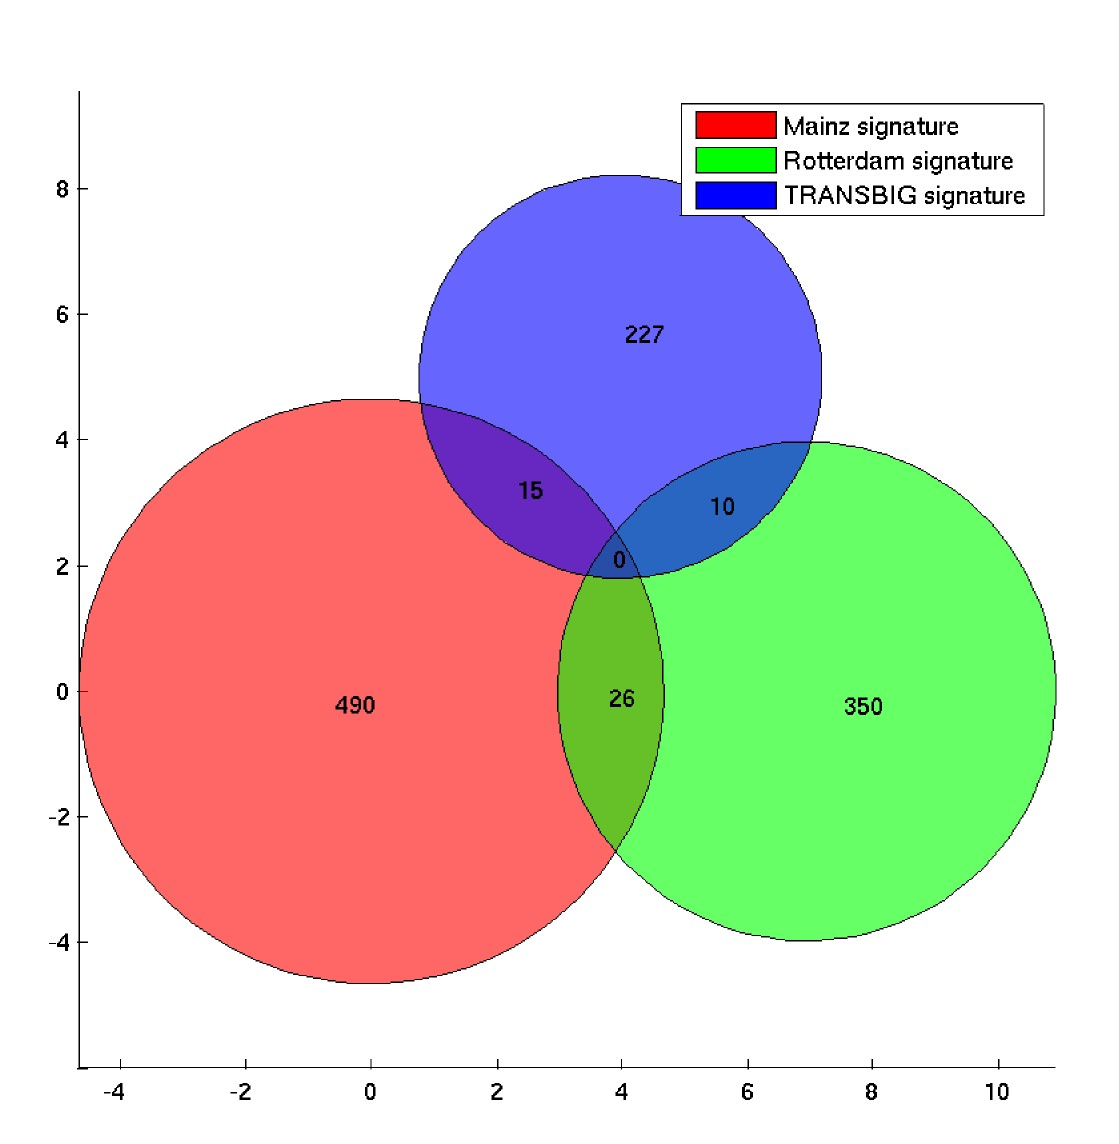
\includegraphics[width=0.65\textwidth]{Figures/SignatureOverlapVenn.jpeg}
\caption{Venn diagram of the probeset content for the three finalised breast cancer signatures.}
\label{Fig:Venn3}
\end{figure}

Indeed the most frequently observed Gene Ontology biological processes shown to be statistically significant ($p < 0.01$) in all three signatures were cell cycle processes, RNA splicing and metabolic processes, all of which may have implications in cancer development. The results for the functional analysis using the KEGG database revealed a number of pathways of interest including the erythropoietin (EPO) signalling pathway which has been shown to influence numerous cellular functions including proliferation, apoptosis, and drug resistance, all of which could possibly contribute towards decreased survival (\citet{Hedley:11}). Genes involved in MAP kinase signalling were also significantly enriched in these signatures. Abnormalities in MAP kinase have been shown to affect most cellular processes required by tumours in order to survive, and thus play a critical role in the development and progression of cancer (\citet{Dhillon:07}). 



\subsection{Prognostic signature validation results}
The final models were applied to the independent validation data sets, yielding c-index values and uncorrected hazard ratios as shown in the off-diagonal entries of Table \ref{Table:HRTable2}. Bootstrap quantile-based 95\% confidence intervals were calculated for the c-index. The confidence intervals for HR were estimated using a $1.96$ standard error interval around the $\ln(HR)$. In terms of the HR confidence intervals not containing the value $1$, the signatures from the Mainz and Rotterdam datasets validate externally. None of the c-index confidence intervals contain the value $0.5$ and therefore all of the signatures validate based on c-index alone.

Correction of the hazard ratios for clinical covariates was not feasible due to different sets of covariates in the three data sets. However, an assessment of the clinical covariate confounding for the validation set predictions is summarised in Table \ref{Table:ValIndep2} in terms of Cox model likelihood ratio test p-values. The p-values for the external validation set predictions were $0.003$ and $0.101$ when using the signature derived from the Mainz data set in predicting Rotterdam and TRANSBIG, respectively. When using the signature derived from the Rotterdam data, the p-values were $0.093$ and $0.002$ for Mainz and TRANSBIG. The higher ($0.101$ and $0.093$) p-values are concordant with low proportional hazards assumption check p-values that indicate a violation of the proportional hazards assumption for these combinations of signatures and validation data; see results below and the discussion section for the implications. The p-values for the predictions from the TRANSBIG dataset model were well above $0.05$ and therefore independence to clinical covariates could not be shown given the samples size.

%%%%%%%%%%%%%%%%%%%%%%%%%%%
%%%%%%%%%%%%%%%%%%%%%%%%%%%

\begin{table}[h]
\centering
\caption{Likelihood ratio test p-values for the breast cancer validation set predictions and clinical covariates (confounders). The p-values are obtained by testing the multivariate Cox model likelihood of the predictions and the clinical covariates in modelling survival time versus reduced models. For each entry in the table the corresponding covariate was dropped and the likelihood ratio p-value of the reduced model was evaluated. Low p-values imply a significant drop in the likelihood.}
\label{Table:ValIndep2}
\begin{small}
    \begin{tabular}{ | l r | l | l | l |} 
    \hline
     & Model & Mainz & Rotterdam & TRANSBIG \\ Data & & 531PS & 386PS & 252PS \\\hline \hline
    Mainz & Predictions:& & 0.093& 0.307\\ &Grade: & & 0.052& 0.035\\ &Size:& & 0.207& 0.136\\\hline
		Rotterdam  & Predictions:& 0.003& & 0.230\\ &ER+: & 0.981& & 0.826\\ &Brain relapse: & 0.0002& & 0.0001\\\hline
		TRANSBIG  & Predictions:& 0.101& 0.002& \\ & Hosp.Guy: & 0.029& 0.004& \\ & Hosp.Igr: & 0.290& 0.127& \\ & Hosp.Jrh: & 0.145& 0.126& \\ & Hosp.Kar: & 0.114& 0.018& \\ & Age:& 0.344& 0.325& \\ & Size: & 0.031& 0.011& \\ & Surgery: & 0.960& 0.735& \\ & Hist.1: & 0.763& 0.446& \\ & Hist.2: & 0.452& 0.179& \\ & Hist.3: & 0.610& 0.474& \\ & Grade:& 0.736& 0.830& \\ &ER+:& 0.287 & 0.272& \\ \hline
    \end{tabular}
\end{small}
\end{table}


The proportional hazards assumption was verified for the dichotomised validation set predictions. The p-values for checking this assumption were evaluated using the correlation between the scaled Schoenfeld residuals for the dichotomised predictions and the ranking of individual follow-up times. Table \ref{Table:HRTable2} shows these p-values were below $0.05$ (indicating a violation) when using either of the Rotterdam or TRANSBIG dataset signatures to predict the Mainz data, as well as when using the Mainz dataset signature in predicting risk of distant metastasis in the TRANSBIG data.

The Kaplan-Meier plots of the validation set predictions are shown in Figure \ref{Fig:PLSCoxKaplanMeier} for the three breast cancer signatures.

The effect of varying the definition of censoring in the TRANSBIG data set on the resulting hazard ratios was also briefly considered. Reducing the censoring threshold from ten to five years increased the HR to $5.12$ and the c-index to $0.667$, compared to $2.55$ and $0.617$ when using the recommended censoring threshold of ten years. Using the data without censoring any events, the HR was just above $1$ and the c-index was $0.602$. See Figure \ref{Fig:PLSCoxKaplanMeierDesmedtVarCensoring} for Kaplan-Meier plots when varying the censoring threshold.

%
% Kaplan-Meier
%
\begin{figure}[!th]
%\vspace*{-2.5cm}
\centering
\subfigure[Model: Mainz, Data: Rotterdam]{
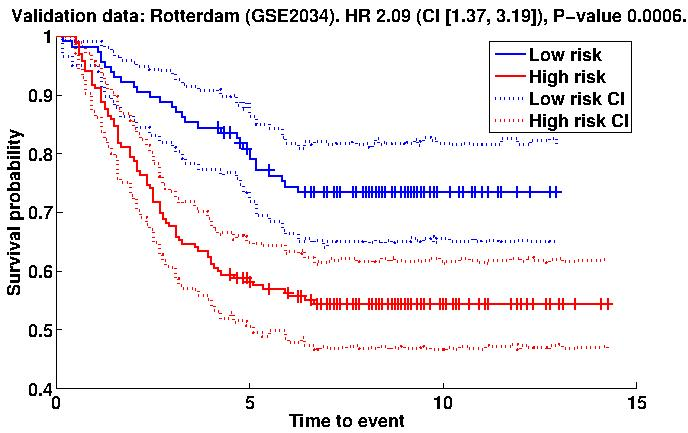
\includegraphics[width=0.48\textwidth]{Figures/Mainz_WangKM.jpeg}
\label{fig:KM1subfig1}
}
\subfigure[Model: Mainz, Data: TRANSBIG]{
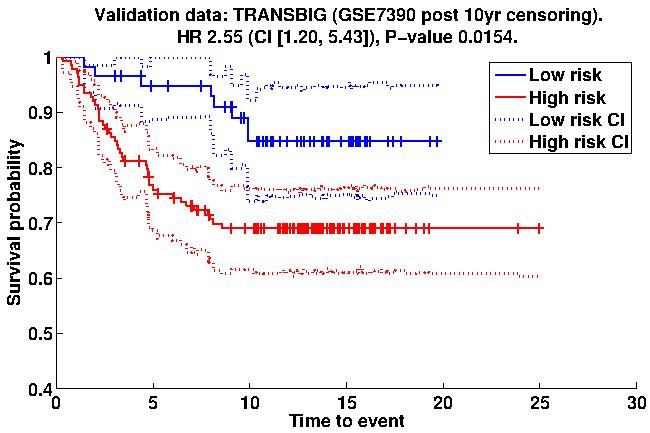
\includegraphics[width=0.48\textwidth]{Figures/Mainz_DesmedtKM10yrCens.jpeg}
\label{fig:KM1subfig2}
}
\subfigure[Model: Rotterdam, Data: Mainz]{
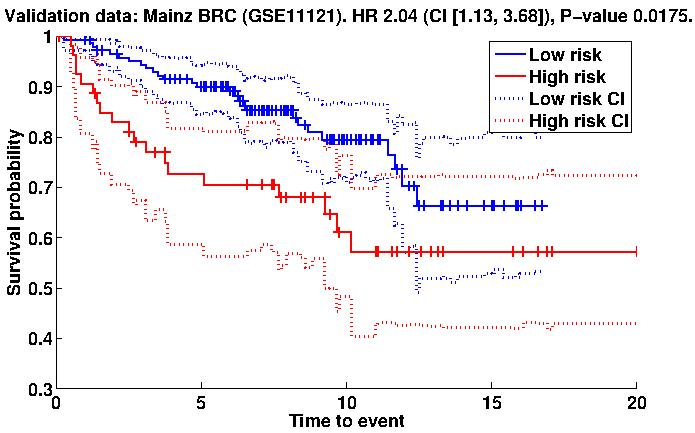
\includegraphics[width=0.48\textwidth]{Figures/Wang_MainzKM.jpeg}
\label{fig:KM2subfig1}
}
\subfigure[Model: Rotterdam, Data: TRANSBIG]{
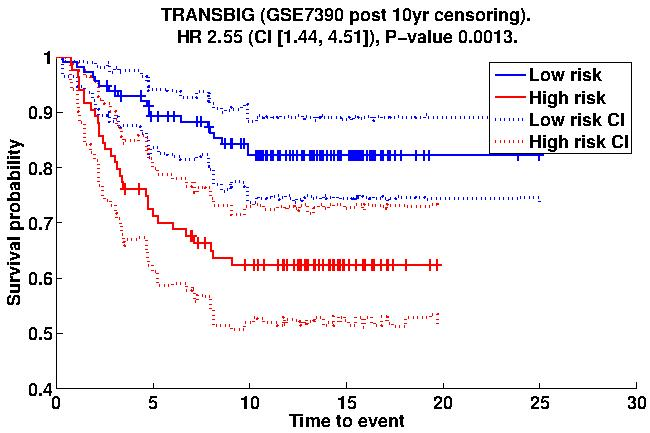
\includegraphics[width=0.48\textwidth]{Figures/Wang_DesmedtKM.jpeg}
\label{fig:KM2subfig2}
}
\subfigure[Model: TRANSBIG, Data: Mainz]{
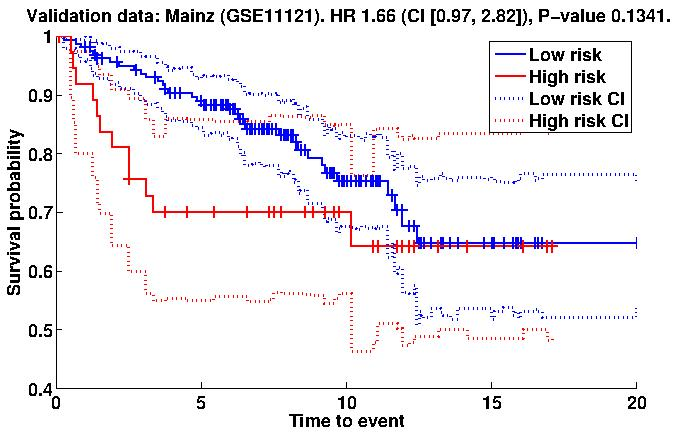
\includegraphics[width=0.48\textwidth]{Figures/Transbig_MainzKM.jpeg}
\label{fig:KM3subfig1}
}
\subfigure[Model: TRANSBIG, Data: Rotterdam]{
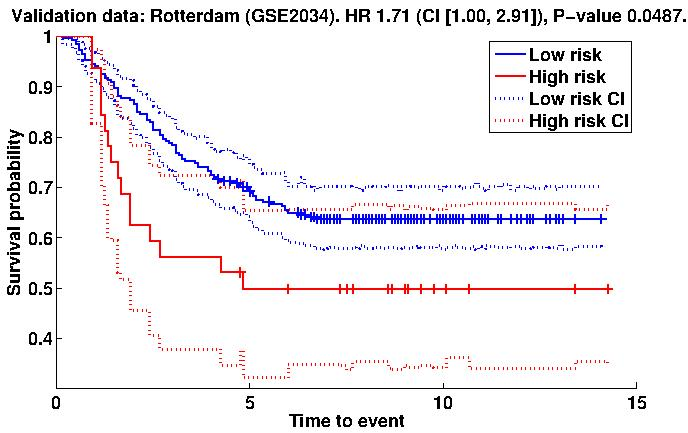
\includegraphics[width=0.48\textwidth]{Figures/Transbig_WangKM.jpeg}
\label{fig:KM3subfig2}
}
\caption{Kaplan-Meier plots of dichotomised validation set predictions. The solid curves represent the predicted low and high risk groups. Bootstrap based 2.5\% and 97.5\% quantiles are shown for the survival probability curves.}
\label{Fig:PLSCoxKaplanMeier}
\end{figure}

% Kaplan-Meier for illustrating instability of HR
\begin{figure}[!th]

\centering
\subfigure[Data: TRANSBIG as-is]{
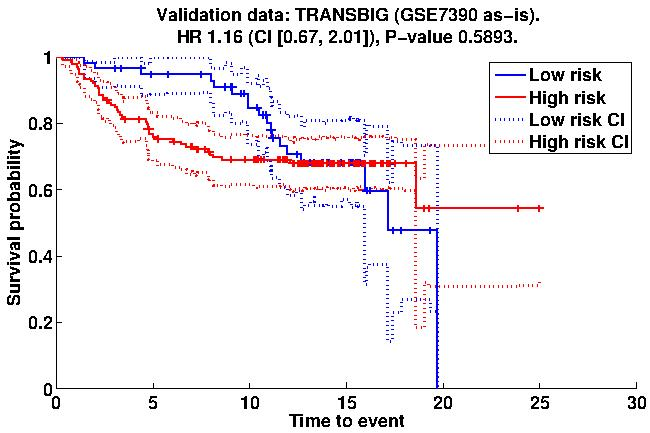
\includegraphics[width=0.48\textwidth]{Figures/Mainz_DesmedtKMUnmod.jpeg}
\label{fig:KM4subfig1}
}
\subfigure[Data: TRANSBIG 5yr censored]{
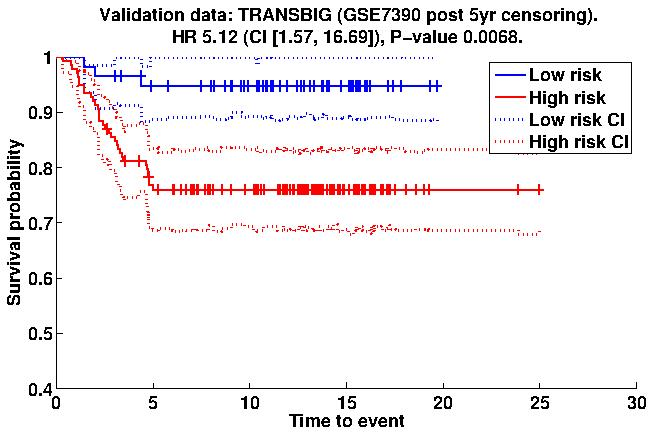
\includegraphics[width=0.48\textwidth]{Figures/Mainz_DesmedtKM5yrCens.jpeg}
\label{fig:KM4subfig2}
}
\caption{Kaplan-Meier plot of dichotomised TRANSBIG data set predictions using the 531 probeset signature generated from the Mainz data. The solid curves represent the predicted low and high risk groups. \subref{fig:KM4subfig1} Data taken as is. \subref{fig:KM4subfig2} All samples with follow-up of more than 5 years censored.}
\label{Fig:PLSCoxKaplanMeierDesmedtVarCensoring}
\end{figure}


\section{Discussion}
In this study we have taken a novel approach to generate multigene signatures using time to event data combined with comprehensive model selection criteria. Primary emphasis in the selection of signatures was placed on the concordance index and the simple univariate hazard ratio of the cross-validation test set predictions, supported by evaluations of biological enrichment and independence from available clinical covariates. 

Using the Mainz dataset for training, a prognostic signature of $531$ probesets was chosen based on performance under cross-validation (see Figures \ref{Fig:PLSCoxCindex}-\ref{Fig:PLSCoxIndep}). This signature validated in the Rotterdam dataset with a HR for risk of distant metastasis following surgery of $2.09 [1.37, 3.19]$ (p-value = $0.0006$) and in the TRANSBIG dataset with a HR of $2.55 [1.20, 5.43]$ (p-value = $0.0154$). Importantly, due to our methodology, the signature performance was independent from known prognostic factors such as tumour size, grade, ER status and age (p-values for predictions in Table \ref{Table:ValIndep2}, column 2, below $0.05$). The performance characteristics of our signature compares favourably to a B-cell metagene that yielded a HR of $1.28$ on Rotterdam data high-grade tumours and HR of $1.2$ on the TRANSBIG data set enriched for younger patients (\citet{Schmidt:08}). 

The Rotterdam dataset was also used to generate a signature of $386$ probesets. This signature validated with a HR for metastatic recurrence of $2.04 [1.13, 3.68]$, (p-value = $0.0175$) and $2.55 [1.44, 4.51]$, (p-value = $0.0013$) in the Mainz and TRANSBIG datasets respectively. This signature was also independent from known prognostic factors in the TRANSBIG dataset (Table \ref{Table:ValIndep2}), indicating clinical utility.

The validation performance of the signatures from both the Mainz and Rotterdam datasets compare favourably with prognostic signatures that have entered clinical practice; the MammaPrint 70 gene signature (\citet{Veer:02}) yielded an unadjusted HR of $2.32$ in external validation (TRANSBIG data, \citet{Buyse:06}) and Oncotype DX achieved an adjusted HR of $2.81$ (\citet{Paik:04}), thereby demonstrating the potential clinical utility of the prognostic signatures generated using our approach.

A $252$ probeset signature was generated from the TRANSBIG dataset. The performance for this signature, however, was inferior to the other two signatures developed here when evaluated in the Mainz and Rotterdam datasets with HR evaluated at $1.66 [0.86, 3.20]$, (p-value = $0.1341$) and $1.71 [1.00, 2.91]$, (p-value = $0.0487$) respectively. The performance was independent from grade and tumour size in the two datasets (Table \ref{Table:ValIndep2}). Although it is unclear why this signature failed to perform as well as the other two, it is interesting to note that the mean patient age was $46$ in TRANSBIG versus $60$ and $54$ in the Mainz and Rotterdam datasets respectively. The greater representation of younger women in the TRANSBIG training set may result in over representation of specific molecular subtypes such as Basal-like tumours (\citet{Millikan:08}) thereby reducing the ability of the signature to validate in older populations. Interestingly The Kaplan-Meier plot in Figure %\ref{fig:KM3subfig1} 
\ref{Fig:PLSCoxKaplanMeier}(a) demonstrates that this signature predicts the outcome in the Mainz dataset until five years after which the performance drops. This may indicate that this signature does not capture the biology representing late recurrence adequately and highlights the risks in dichotomising a population based on an arbitrary time point to develop a prognostic signature. 

One of the key assumptions in the Cox model is that of proportional hazards (PH). In a regression setting this means that the survival and hazard curves for the predicted risk groups must be parallel over time, i.e.\ these curves must not cross. For a quantitative test, we used the Schoenfeld residuals from the Cox model to test this proportionality, where a p-value $< 0.05$ (relationship between residuals and time) means that the proportional hazards assumption should be rejected and we cannot rely on the ratio of the hazard functions being accurate. Therefore, when these assumptions are violated, alternative measures such as the c-index give a more accurate measure of signature performance in this setting, since it does not rely on these assumptions.

The PH assumption check (Table \ref{Table:HRTable2}) confirms that in some cases there was a reason to doubt the assumption with respect to the predicted dichotomised risk. The PH test p-values for the dichotomised predictions from the Rotterdam and TRANSBIG data based signatures were below $0.05$ for prediction upon the Mainz patient samples. Similarly, the PH test p-value when using the Mainz data based signature in prediction of the TRANSBIG data was smaller than $0.05$. In these cases the c-index is likely to give a better view of the predictive performance as it is a rank correlation based measure and does not depend on the proportional hazards assumption. This is clearly illustrated in the Kaplan-Meier plot in Figure \ref{Fig:PLSCoxKaplanMeierDesmedtVarCensoring}(a)%\ref{fig:KM4subfig1}
, where the signature initially stratified the patients well (c-index greater than $0.6$) but the PH assumption is violated and HR is very close to one. Consequently we advocate that hazard ratios should always be accompanied by the corresponding PH check p-values and c-index values. In all of the three breast cancer signatures the average c-index under cross-validation was approximately $0.67$ and the validation set c-index values between $0.61$ and $0.65$, showing only a minor positive bias between cross-validation and independent validation. Factors influencing the observed minor drop from cross-validation to validation may include differences in population, laboratories, reagents and temporal differences. 

\section{Conclusions}
In this paper we presented rigorous model selection criteria and developed a semi-automated signature generation framework that was used to discover prognostic multigene assays using time to event data. To facilitate model selection between different signature lengths and conditions, we applied four model selection criteria in parallel, namely the concordance index, hazard ratio, independence from clinical covariates and biological enrichment of the signature genes. Considering multiple criteria in parallel aided in selecting signatures that validated externally, as is evident from the results across the three breast cancer data sets.  We now plan to test this methodology using multi-analyte data generated by other technologies that are entering mainstream molecular profiling such as next-generation sequencing, metabolomics arrays and protein arrays, and also work on shortening the signatures using forward feature selection methods.




%%%%%%%%%%%%%%%%%%%%%%%%%%%%%%%%%%%
%%                               %%
%% Tables                        %%
%%                               %%
%%%%%%%%%%%%%%%%%%%%%%%%%%%%%%%%%%%


%%%%%%%%%%%%%%%%%%%%%%%%%%%%%%%%%%%
%%                               %%
%% Figures                       %%
%%                               %%
%%%%%%%%%%%%%%%%%%%%%%%%%%%%%%%%%%%



%% BibTeX support
\bibliographystyle{DeGruyter}
\bibliography{TimeToEvent}

\end{document}
